\documentclass[12pt,-letter paper]{article}
\title{\textbf{MATHS PAPERS}}
\usepackage{siunitx}
\usepackage{setspace}
\usepackage{gensymb}
\usepackage{xcolor}
\usepackage{caption}
%\usepackage{subcaption}
\doublespacing
\singlespacing
\usepackage[none]{hyphenat}
\usepackage{amssymb}
\usepackage{relsize}
\usepackage[cmex10]{amsmath}
\usepackage{mathtools}
\usepackage{amsmath}
\usepackage{commath}
\usepackage{amsthm}
\interdisplaylinepenalty=2500
%\savesymbol{iint}
\usepackage{txfonts}
%\restoresymbol{TXF}{iint}
\usepackage{wasysym}
\usepackage{amsthm}
\usepackage{mathrsfs}
\usepackage{txfonts}
\let\vec\mathbf{}
\usepackage{stfloats}
\usepackage{float}
\usepackage{cite}
\usepackage{cases}
\usepackage{subfig}
%\usepackage{xtab}
\usepackage{longtable}
\usepackage{multirow}
%\usepackage{algorithm}
\usepackage{amssymb}
%\usepackage{algpseudocode}
\usepackage{enumitem}
\usepackage{mathtools}
%\usepackage{eenrc}
%\usepackage[framemethod=tikz]{mdframed}
\usepackage{listings}
%\usepackage{listings}
\usepackage[latin1]{inputenc}
%%\usepackage{color}{   
%%\usepackage{lscape}
\usepackage{textcomp}
\usepackage{titling}
\usepackage{hyperref}
%\usepackage{fulbigskip}   
\usepackage{tikz}
\usepackage{graphicx}
\lstset{
  frame=single,
  breaklines=true
}
\let\vec\mathbf{}
\usepackage{enumitem}
\usepackage{graphicx}
\usepackage{siunitx}
\let\vec\mathbf{}
\usepackage{enumitem}
\usepackage{graphicx}
\usepackage{enumitem}
\usepackage{tfrupee}
\usepackage{amsmath}
\usepackage{amssymb}
\usepackage{mwe} % for blindtext and example-image-a in example
\usepackage{wrapfig}
\graphicspath{{figs/}}
\providecommand{\mydet}[1]{\ensuremath{\begin{vmatrix}#1\end{\vmatrix}}}
\providecommand{\myvec}[1]{\ensuremath{\begin{bmatrix}#1\end{\bmatrix}}}
\providecommand{\cbrak}[1]{\ensuremath{\left\{#1\right\}}}
\providecommand{\brak}[1]{\ensuremath{\left(#1\right)}}
\begin{document}
\maketitle
\section*{DISCRETE}
\begin{enumerate}
\item
\textbf{Assertion$\brak{A}$:}$a,b,c$ are in $A.P.$ if and if only if $2b = a + c$.

\textbf{Reason$\brak{R}$:}The sum of first $n$ natural numbers is $n^2$.
\begin{enumerate}
\item Both Assertion $\brak{A}$ and Reason $\brak{R}$ are true and Reason $\brak{R}$ is the correct explanation of Assertion $\brak{A}$.
\item Both Assertion $\brak{A}$ and Reason $\brak{R}$ are true and Reason $\brak{R}$ is not the correct explanation of Assertion $\brak{A}$.
\item Assertion $\brak{A}$ is true but Reason $\brak{R}$ is false.
\item Assertion $\brak{A}$ is false but Reason $\brak{R}$ is true.
\end{enumerate}
\item
How many terms are there in $A.P.$ whsoe first and fifth term are $-14$ and $2$, respectively and the last term is $62$.
\item
Which term of the $A.P.$ : $65,61,57,53, ..................$ is the first negative term?
\section*{POLYNOMIAL EQUATIONS}
\item
Find the sum and product of the roots of the quadratic equation $2x^2-9x+4=0$.

\item
Find the discriminant of the quadratic equation $4x^2-5=0$ and hence comment on the nature of roots of the equation.
\item
If one zero of polynomial $p$\brak{x}$=6x^2+37x-\brak{k-2}$ is reciprocal of the other, then  find the value of $k$.
\item
Find the value of $'p'$ for which one root of the quadratic equation $px^2-14x+8=0$ is $6$ times the other.
\section*{TRIGNOMETRY}
\item
Evaluate \begin{align}
2\sec^2\theta + 3\csc^2\theta - 2\sin\theta\cos\theta  \ \text{if} \ \theta = 45\degree.
\end{align}
\item 
If \begin{align} 
\sin\theta - \cos\theta = 0, \text{ then find the value of }\sin^4\theta + \cos^4\theta.
\end{align}
\item
Prove that \begin{align} \frac{\sin{A}-2sin^3{A}}{2\cos^3{A}-\cos{A}}=\tan{A} \end{align}
\item
Prove that \begin{align} \sec{A\brak{1-\sin{A}}\brak{\sec{A}+\tan{A}}}=1. \end{align}
\item
	A straight highway leads to the foot of a tower. A man standing on the top of the $75 \mathrm{m}$ high tower observes two cars at angles of depression of $30^\circ$ and $60^\circ$, which are approaching the foot of the tower. If one car is exactky behind the other on the same side of the tower, find the dist
ance between the two cars. use \brak{\sqrt{3}=1.73}.
\item
	From the top of a $7 \mathrm{m}$ building, the angle of elevation of the top a cable tower is 60\degree and the angle of depression of its foot is 30\degree. Determine the height of the tower.
\section*{GEOMETRY}
\item
From an external point, two tangents are drawn to a circle. Prove that the line joining the external point to the center of the circle bisects the angle between the two tangents.
\item
	Two concentric circles are of radii $5\mathrm{cm}$and $3\mathrm{cm}$. Find the length of the chord of the larger circle which touches the smaller circle.
\item
In a $\triangle{PQR}$, $N$ is a point on $PR$, such that $QN$$\perp$$PR$. If $PN \times NR=QN^2$, prove that $\angle{PQR}=90^{\circ}$.
\newpage
\item
In the given figure, $\triangle ABC$  and  $\triangle$ $DBC$  are on the same base $BC$.  $AD$ intersects $BC$ at $O$.
prove that  $\frac{\text{ar}\brak{\triangle ABC}}{\text{ar}\brak{\triangle DBC}} = \frac{AO}{DO}$
\begin{figure}[h!]
\centering
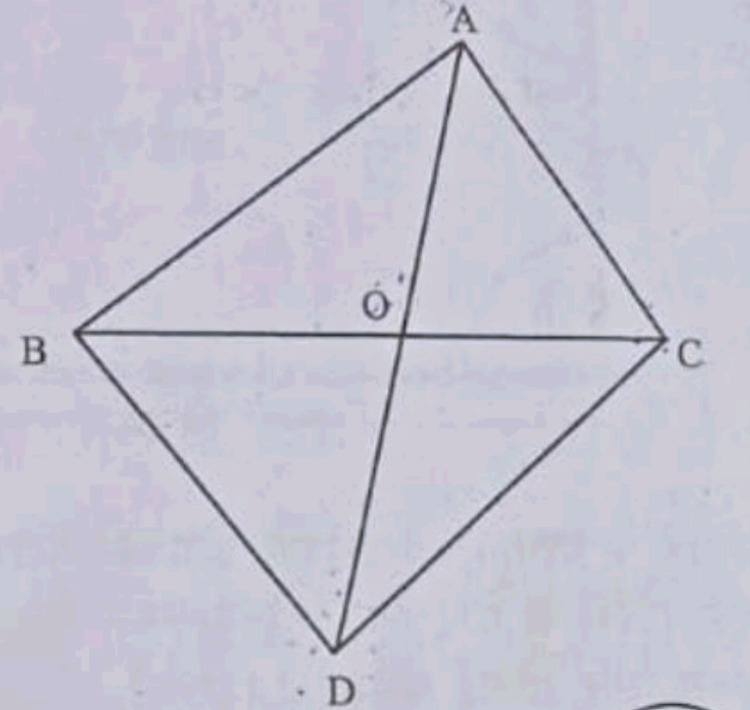
\includegraphics[width=\columnwidth]{img1.jpg}
\caption{Image 1}
\end{figure} 
\newpage
\item
	A wooden article was made by scooping out a hemisphere from each end of a solid cylinder, as shown in the figure. If the height of the cylinder is $10\mathrm{cm}$ and its base is of radius $3.5\mathrm{cm}$, find the total surface area of the article.
\begin{figure}[h!]
\centering
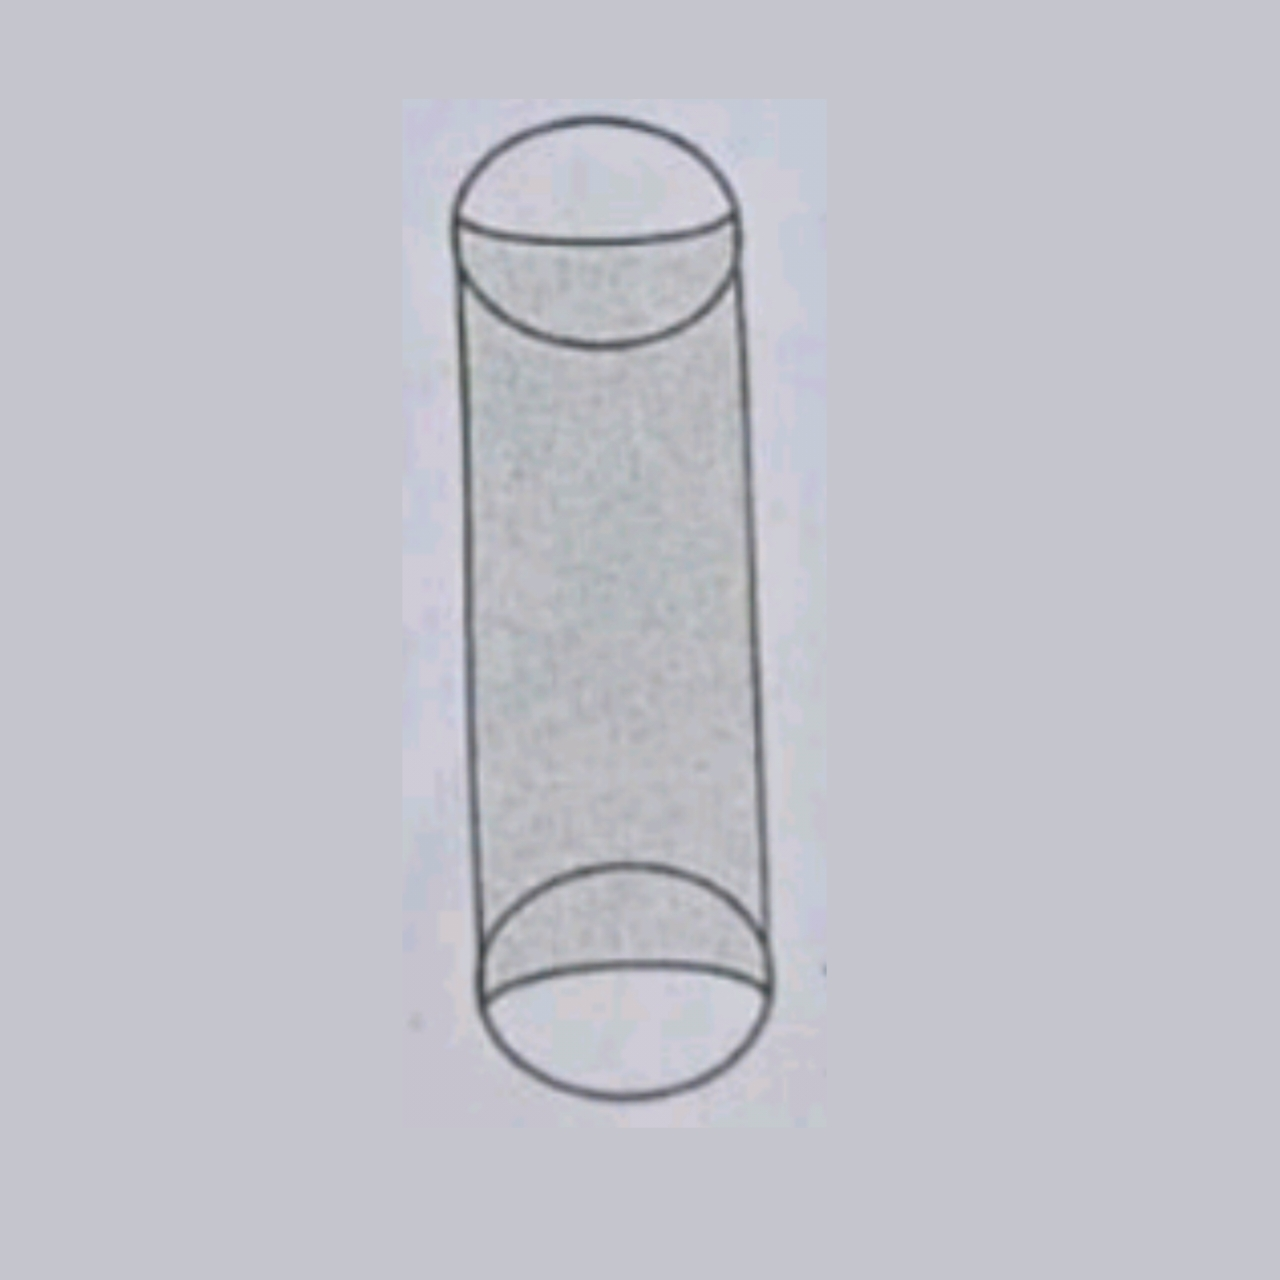
\includegraphics[width=\columnwidth]{img2.jpg}
\caption{Image 2}
\end{figure}
\newpage
\item
Governing council of a local publc development authority of Dehradun decided to build an adventurous playground on the top of a hill, which will have adequate space for parking.
\begin{figure}[h!]
\centering
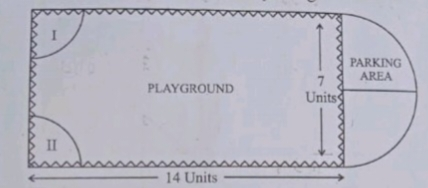
\includegraphics[width=\columnwidth]{img3.jpg}
\caption{Image 3}
\end{figure}
After survey, it was decide to build rectangular playground, with a semi-circular area allotted for parking at one one end of the playground. The length and breadth of the rectangular playground are $14$ units and $7$ units, respectively. There are two quadrants of radius $2$ units on one side for s
pecial seats.
Based on the above information, answer the following questions:
\begin{enumerate}
\item
What is the total perimeter of the parking area?
\item
\begin{enumerate}
\item
What is the total area of parking and the two quadrants?
\item
Whast is the ratio of area of playground to the area of paarking area?
\end{enumerate}
\item
Find the cost of fencing the playground and parking area at the rate of \rupee $2$ per unit.
\newpage
\item
Two schools $P$ and $Q$ decided to award prizes to their students for two games of Hockey \rupee $x$ per student and Cricket \rupee $y$ per student. School $P$ decided to award a total of \rupee $9,500$ for the two games to $5$ and $4$ students respectively; while school $Q$ decided to award
 \rupee $7,370$ for the two games to $4$ and $3$ students respectively.
\begin{figure}[h!]
\centering
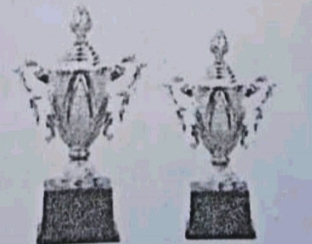
\includegraphics[width=\columnwidth]{img4.jpg}
\caption{Image 4}
\end{figure}
Based on the given information,answer the following questions:
\begin{enumerate}
\item
Represent the following information in algebraically (in terms of $x$ and $y$).
\item
\begin{enumerate}
\item
What is the prize amount for hockey?
\item
Prize amount on which game is more and by how much?
\end{enumerate}
\item
What will be the total prize amount if there are $2$ students each from two games?
\end{enumerate}
\end{enumerate}
\newpage
\item
Jagadish has a field which is in the shape of a right angled triangle $AQC$. He wants to leave a space in the form of a square $PQRS$ inside the field for growing wheat and the remaining for growing vegetables \brak{as shown in the figure}. In the field, there is a pole marked as $O$.
\begin{figure}[h!]
\centering
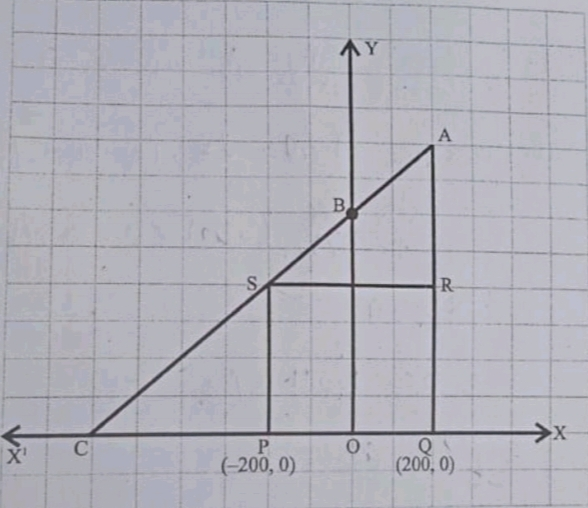
\includegraphics[width=\columnwidth]{img5.jpg}
\caption{Image 5}
\end{figure}
Based on the above information, answer the following questions:
\begin{enumerate}
\item
Taking $O$ as origin, coordinates of $P$ are \brak{-200,0} and of $Q$ are \brak{200,0}. $PQRS$ being a square, what are the coordinates of $R$ and $S$?
\item
\begin{enumerate}
\item
What is the area of square $PQRS$?
\item
What is the length of diagonal $PR$ in square $PQRS$?
\end{enumerate}
\item
If $S$ divides $CA$ in the ratio $K:1$, what is the value of $K$, where point $A$ is \brak{200,800}?
\end{enumerate}
\section*{PROBABILITY}
\item
If a fair coin is tossed twice, find the probability of getting atmost one head.
\section*{NUMBER SYSYTEM}
\item
Two numbers are in the ratio $2:3$ and their $LCM$ is $180$. What is the $HCF$ of these numbers?
\item
Prove that $\sqrt{5}$ is an irrational number.
\section*{STATISTICS}
\item
The monthly expenditure on milk in $200$ families of a Housing Society is given below:\\
\\
\footnotesize
\setlength{\tabcolsep}{1pt}
\begin{tabular}{|l|c|c|c|c|c|c|c|c|}
\hline
	Monthly Expenditure \brak{in \rupee} & 1000-1500 & 1500-2000 & 2000-2500 & 2500-3000 & 3000-3500 & 3500-4000 & 4000-4500 & 4500-5000 \\ \hline
Number of Families & 24 & 40 & 33 & $x$ & 30 & 22 & 16 & 7 \\ \hline
\end{tabular}\\

Find the value of $x$ and also, find the median and mean expenditure on milk.



\end{enumerate}
\end{document}

